\chapter{Resultados}
\label{chap:resultados}

Para exemplificação do uso do sistema proposto na prática, foram desenvolvidos alguns projetos de exemplo. Devido a dificuldade na implementação de uma planta completa com dispositivos normalmente encontrados na Indústria, foram utilizados microcontroladores para gerar as informações disponíveis nas seções abaixo que trarão os mesmos efeitos caso fossem utilizados dispositivos industriais com conexão à \textit{internet}.

\section{Temperatura e Umidade}
\label{sec:temperatura-umidade}

Este exemplo tem por objetivo a utilização de variáveis de ambiente em simulação de um processo industrial que fosse necessário o acompanhamento de informações de temperatura e umidade. Foram utilizados os seguintes materiais: (i) Placa de desenvolvimento com microcontrolador ESP8266 da fabricante \textit{espressif}, visto na Figura \ref{fig:figura-nodemcu} e (ii) Módulo com sensor de temperatura e umidade DHT11 da fabricante chinesa \textit{Aosong Electronics Co. Ltd}, visto na Figura \ref{fig:figura-dht11}.

O código para este exemplo, anexo \ref{an:anexo-temperatura-umidade}, foi desenvolvido através da linguagem de programação C++ adaptada ao \textit{Arduino} e os dados são transmitidos ao rscada utilizando o protocolo \gls{MQTT}, devido ser a forma de comunicação mais leve para um pequeno dispositivo como o microcontrolador utilizado.

        \begin{figure}[!h]
		\Caption{\label{fig:figura-nodemcu} Placa de desenvolvimento com microcontrolador ESP8266 da fabricante \textit{espressif}.}
		%\centering
		\UFCfig{}{
			\fbox{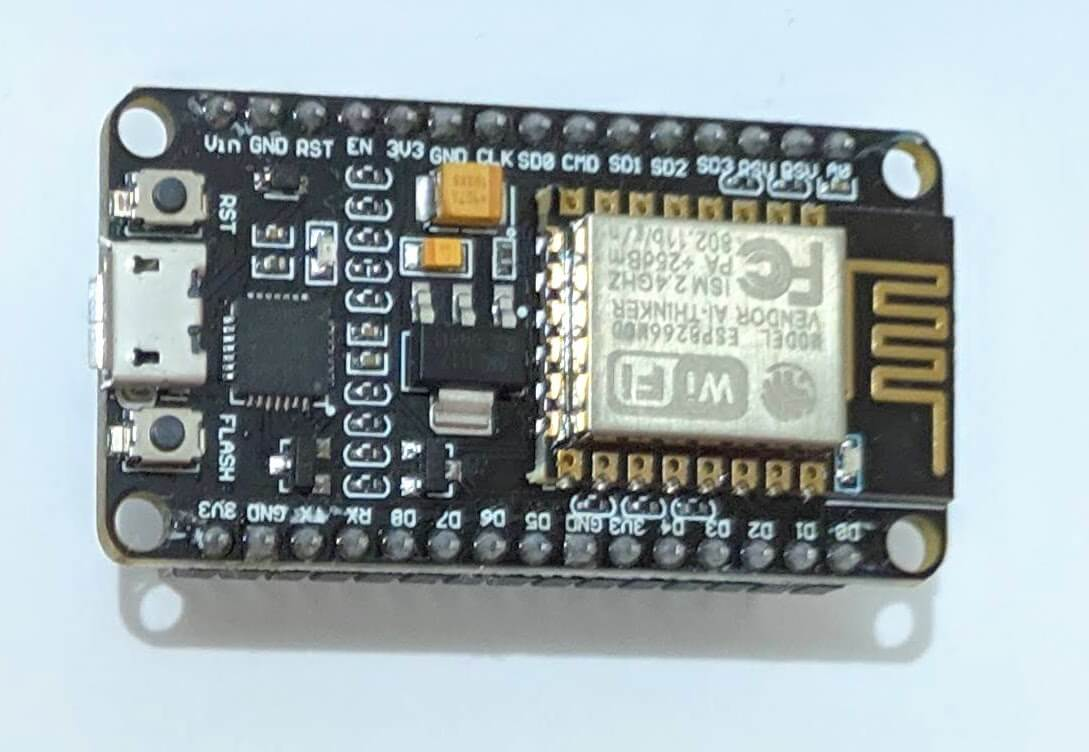
\includegraphics[width=5cm]{figuras/nodemcu.jpg}}
		}{
			\Fonte{O autor}
		}	
    	\end{figure}
    	
    	\begin{figure}[!h]
		\Caption{\label{fig:figura-dht11} Módulo com sensor de temperatura e umidade DHT11.}
		%\centering
		\UFCfig{}{
			\fbox{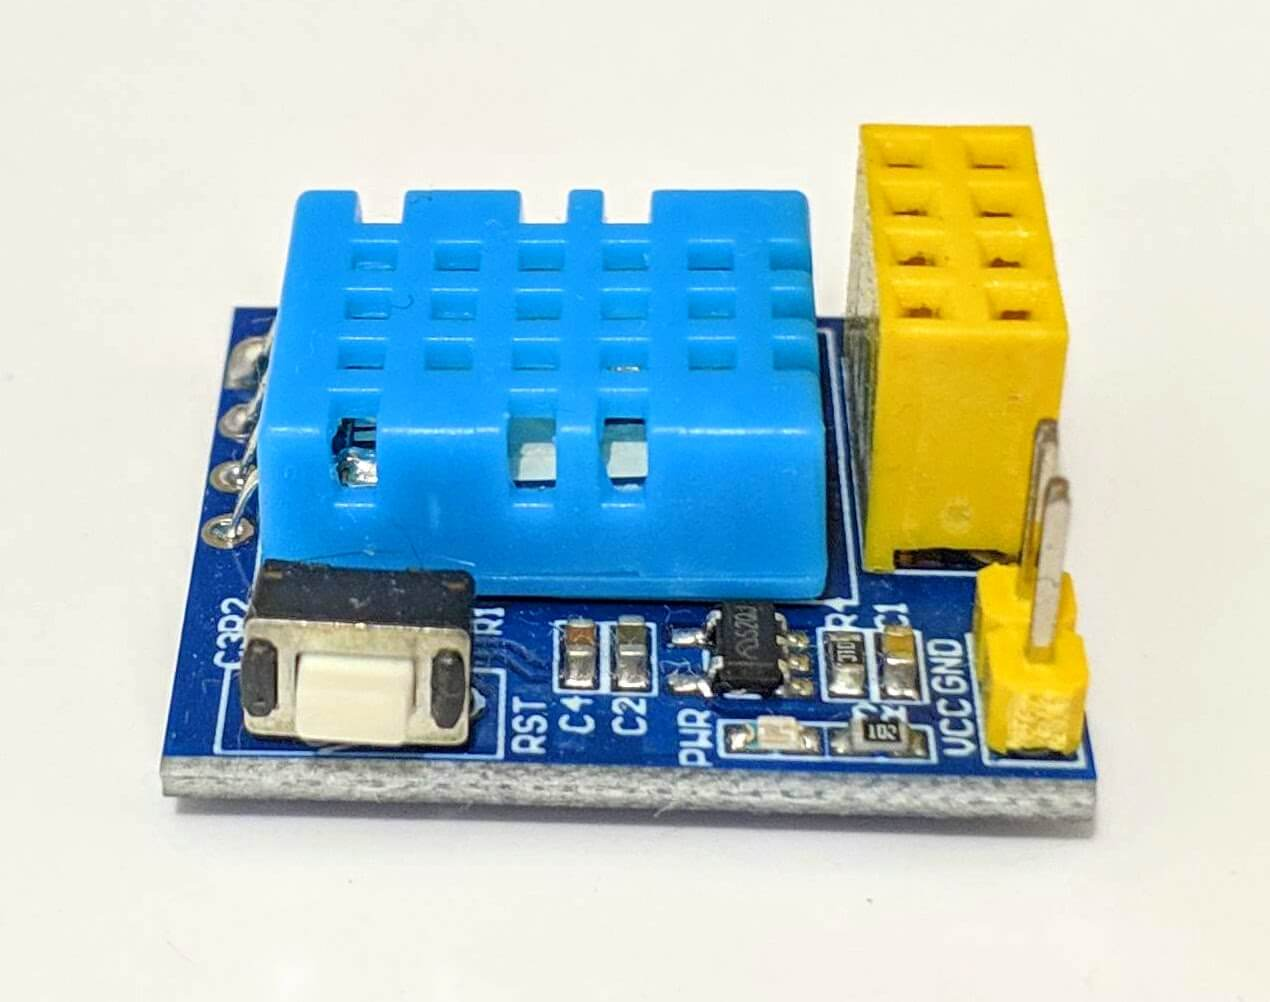
\includegraphics[width=5cm]{figuras/modulo-dht11.jpg}}
		}{
			\Fonte{O autor}
		}	
		
    	\end{figure}
    	
Inicialmente foram configuradas as variáveis à serem utilizadas pelo programa do microcontrolador, sendo elas: (i) Latência, representando o tempo de atraso entre o envio da informação e a resposta do servidor, (ii) Temperatura e (iii) Umidade, ambas do tipo numérica já que representarão números inteiros ou irracionais. A Figura \ref{fig:figura-temperatura-variaveis} traz uma captura da tela de gerenciamento de variáveis, com o exemplo já em funcionamento e um histórico com mais de 4 milhões de pontos de informação em cada variável.

        \begin{figure}[!h]
		\Caption{\label{fig:figura-temperatura-variaveis} Variáveis utilizadas para o projeto.}
		%\centering
		\UFCfig{}{
			\fbox{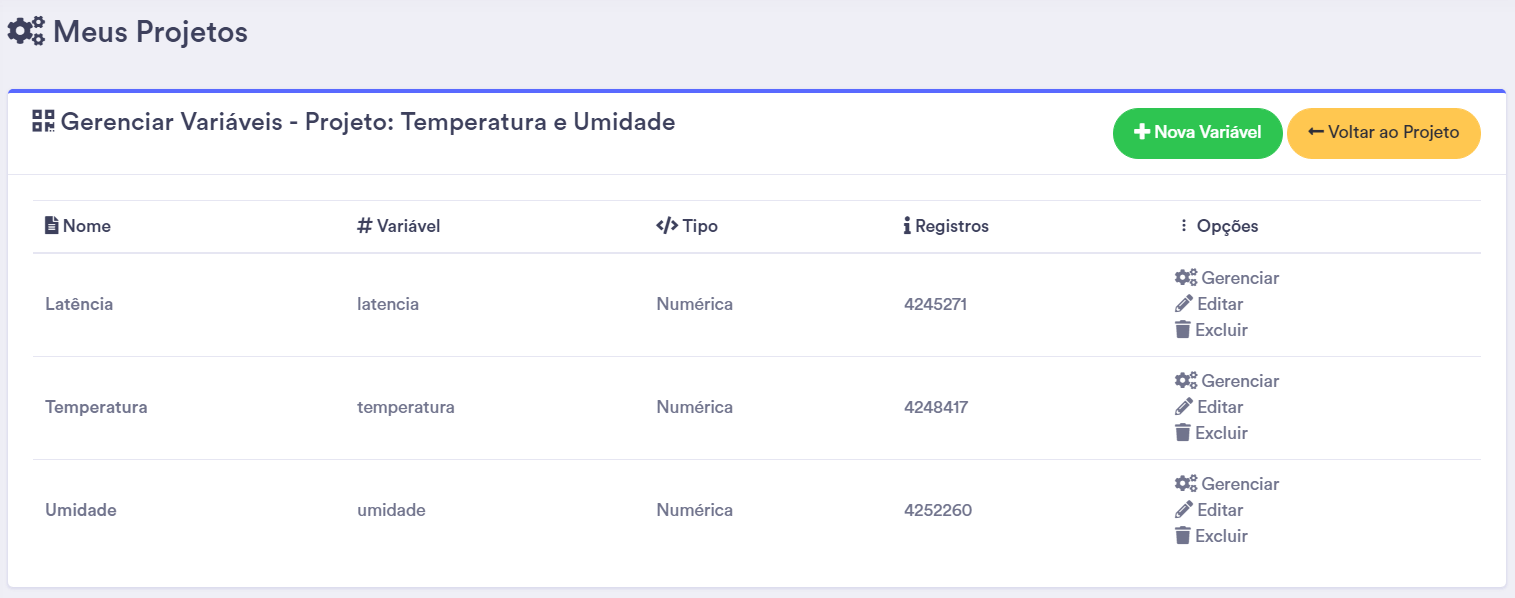
\includegraphics[width=15cm]{figuras/temperatura-variaveis.png}}
		}{
			\Fonte{O autor}
		}	
    	\end{figure}
    	
Para este exemplo foram utilizados um total de 6 objetos, sendo os 3 primeiros do tipo Últimor Valor para demonstrar os valores instantâneos recebidos pelo microcontrolador e suas variações, representados na Figura \ref{fig:figura-temperatura-instataneos} e outros 3 do tipo gráfico, para acompanhar a variação das informações através do tempo em uma janela de tempo configurada com 30 minutos de período. As Figuras \ref{fig:figura-temperatura-grafico} e  \ref{fig:figura-temperatura-umidade} representam os objetos: temperatura e umidade, do tipo Gráfico de Área e a Figura \ref{fig:figura-temperatura-latencia}, a latência da conexão, do tipo Gráfico de Linha.

        \begin{figure}[!h]
		\Caption{\label{fig:figura-temperatura-instataneos} Últimas informações enviadas.}
		%\centering
		\UFCfig{}{
			\fbox{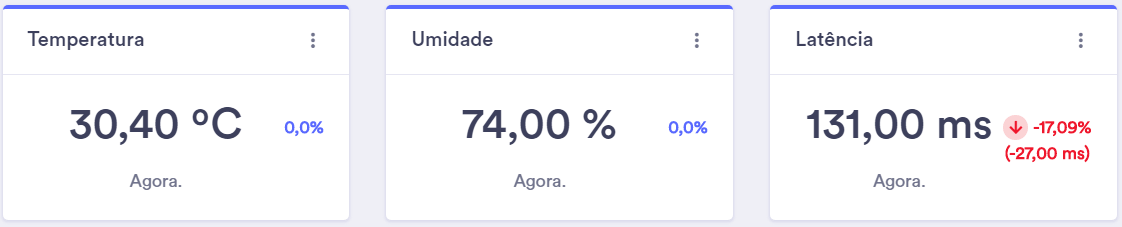
\includegraphics[width=15cm]{figuras/temperatura-instataneos.png}}
		}{
			\Fonte{O autor}
		}	
    	\end{figure}
    	
Os objetos do tipo Último Valor, na Figura \ref{fig:figura-temperatura-instataneos}, foram utilizados para representar os valores instantâneos das variáveis principais do processo, neles, são disponibilizadas as informações sobre há quanto tempo foi enviado o último dado e qual sua variação, em ambos os casos ocorre um alerta caso a temperatura ultrapasse um valor pré-definido ou não tenha a inserção de novos dados durante um dado tempo.

        \begin{figure}[!h]
		\Caption{\label{fig:figura-temperatura-grafico} Gráfico de área com os últimos 30 minutos de temperatura registrada.}
		%\centering
		\UFCfig{}{
			\fbox{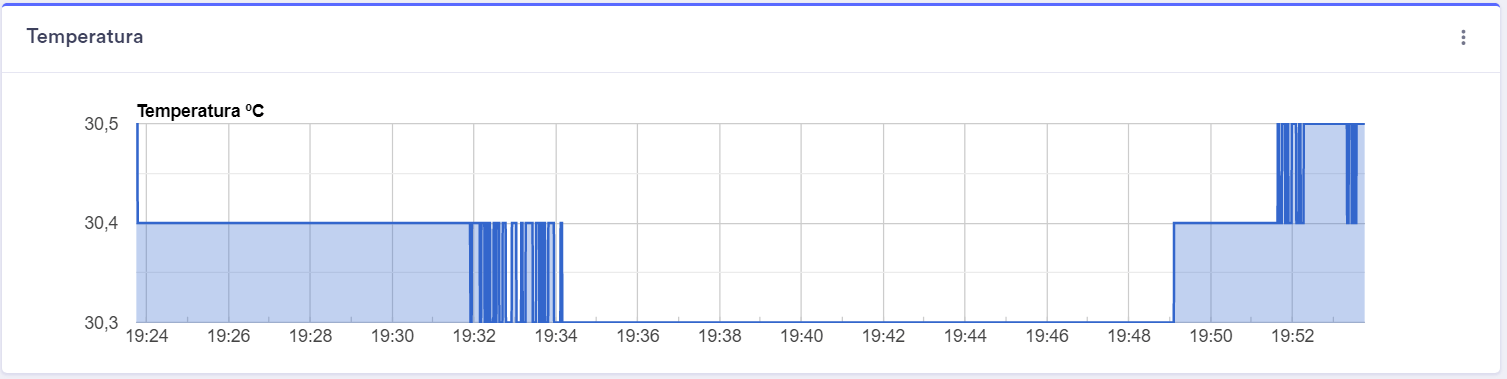
\includegraphics[width=15cm]{figuras/temperatura-grafico.png}}
		}{
			\Fonte{O autor}
		}	
    	\end{figure}
    	
Para o período de captura utilizado neste exemplo, Figura \ref{fig:figura-temperatura-grafico}, houve um intervalo de temperatura entre 30,3 e 30,5ºC, onde a precisão da medição do modelo de sensor utilizado é na casa de 0,1ºC. Devido um parâmetro configurado no gráfico, as amplitudes de temperatura não são demonstradas desde o ponto zero, mas sim, somente entre a temperatura mínima e a máxima, tornando fácil a identificação destes extremos na janela de tempo escolhida. O Gráfico de umidade, representado na Figura \ref{fig:figura-temperatura-umidade}, foi parametrizado seguindo as mesmas observações feitas anteriormente, revelando uma oscilação no mesmo período de tempo da figura anterior, entre 71 e 74\% de umidade relativa do ar com uma precisão do sensor na casa de 1\%.

        \begin{figure}[!h]
		\Caption{\label{fig:figura-temperatura-umidade} Gráfico de área com os últimos 30 minutos de umidade registrada.}
		%\centering
		\UFCfig{}{
			\fbox{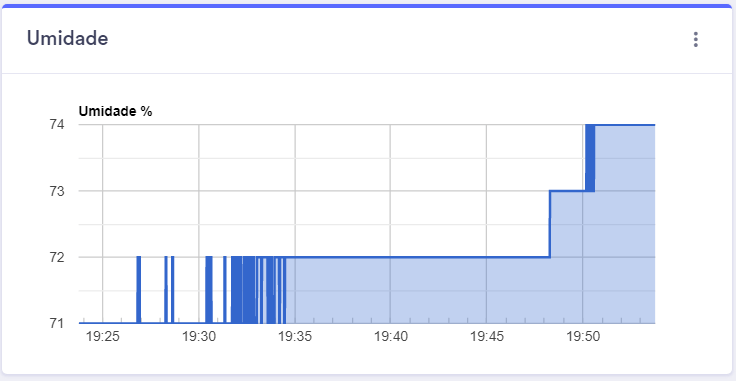
\includegraphics[width=10cm]{figuras/temperatura-umidade.png}}
		}{
			\Fonte{O autor}
		}	
    	\end{figure}
    	
O acompanhamento da latência da conexão entre o microcontrolador e o servidor também foi feito, para que possíveis erros de medição ou atrasos, fossem facilmente identificados. Na Figura \ref{fig:figura-temperatura-latencia}, é possível perceber um leve aumento na latência entre 19h52 e 19h54 do dia em que a captura foi feita, provavelmente devido ao pico de demanda do provedor neste horário.
    	
        \begin{figure}[!h]
		\Caption{\label{fig:figura-temperatura-latencia} Gráfico de linhas com os últimos 30 minutos de latência registrada.}
		%\centering
		\UFCfig{}{
			\fbox{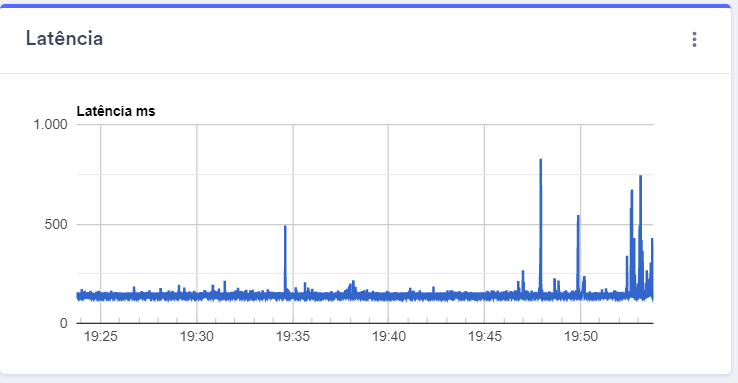
\includegraphics[width=10cm]{figuras/temperatura-latencia.png}}
		}{
			\Fonte{O autor}
		}	
    	\end{figure}
\section{Qualidade Sinal - WiFi}
\label{sec:qualidade-sinal}

O objetivo deste segundo exemplo é acompanhar os níveis de qualidade de sinal, como: potência do sinal recebido e latência da conexão de uma rede  \textit{Wi-Fi} doméstica e um teste com o botão liga/desliga para o controle do status do monitoramento. Para este projeto foi utilizada uma placa de desenvolvimento com microcontrolador ESP32 da fabricante \textit{espressif}, vista na Figura \ref{fig:figura-esp32}, que já possui integrado de fábrica o modem \textit{Wi-Fi}.

O código para este exemplo, anexo \ref{an:anexo-wifi}, também foi desenvolvido através da linguagem de programação C++ adaptada ao \textit{Arduino} e os dados são transmitidos ao rscada utilizando o protocolo \gls{MQTT}, assim como o exemplo anterior, devido ser a forma de comunicação mais leve para um pequeno dispositivo como o microcontrolador utilizado.

        \begin{figure}[!h]
		\Caption{\label{fig:figura-esp32} Placa de desenvolvimento com microcontrolador ESP32 da fabricante \textit{espressif}.}
		%\centering
		\UFCfig{}{
			\fbox{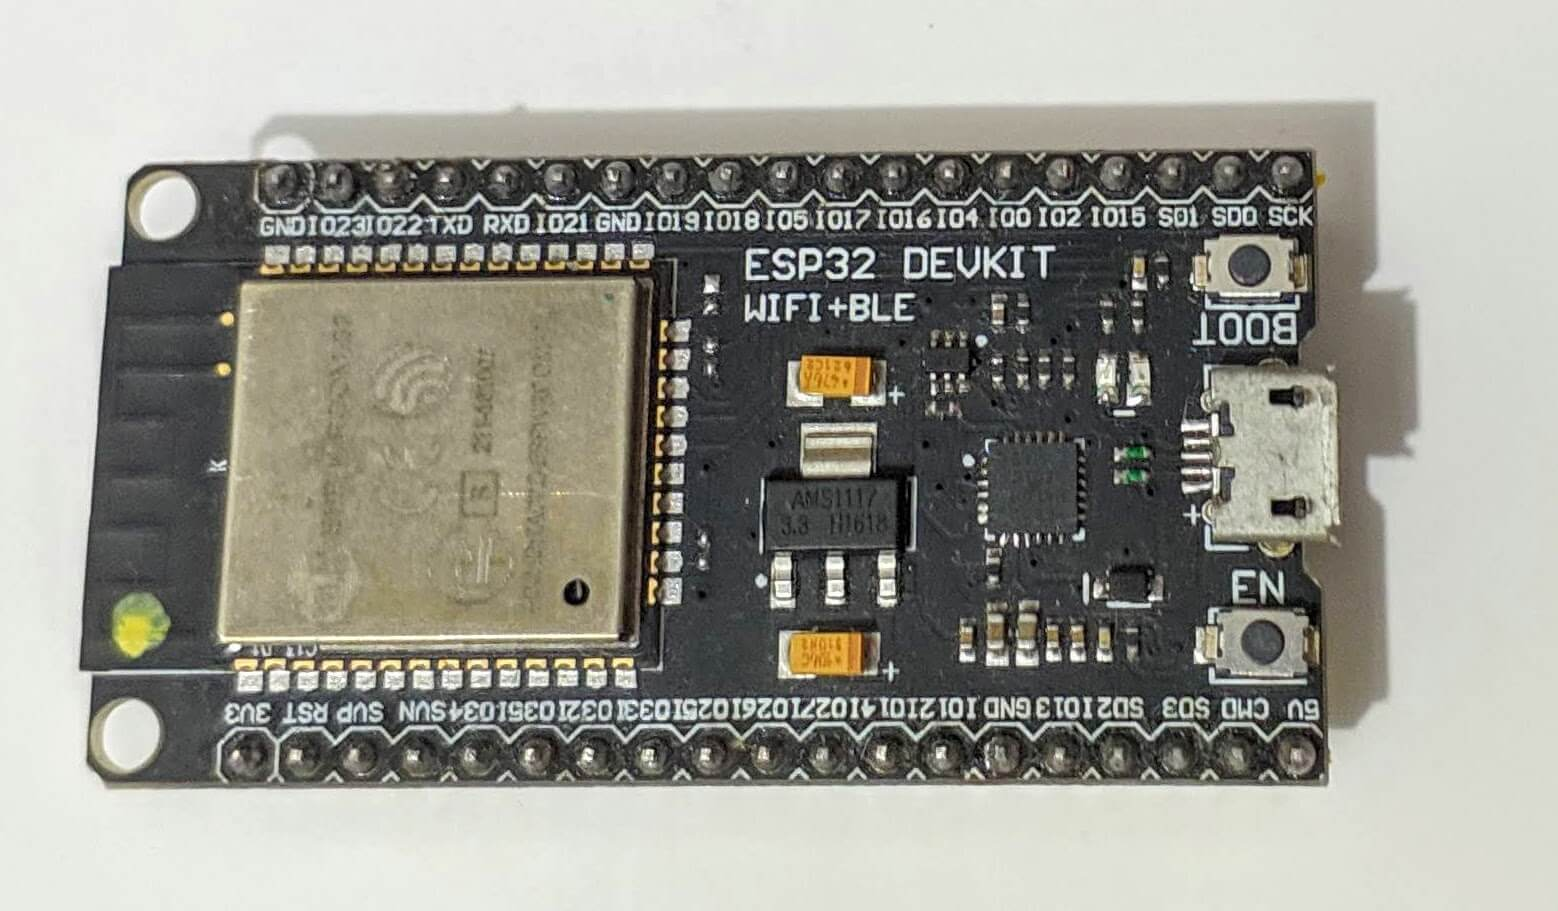
\includegraphics[width=5cm]{figuras/esp32.jpg}}
		}{
			\Fonte{O autor}
		}	
    	\end{figure}
    	
Inicialmente foram configuradas as variáveis à serem utilizadas pelo programa do microcontrolador, sendo elas: (i) Monitoramento, uma variável do tipo binária para o controle da chave liga/desliga, (ii)  Latência, representando o tempo de atraso entre o envio da informação e a resposta do servidor e (iii) Nível de Sinal, ambas do tipo numérica já que representarão números inteiros ou irracionais. A Figura \ref{fig:figura-wifi-variaveis} traz uma captura da tela de gerenciamento de variáveis, com o exemplo já em funcionamento e um histórico com mais de 4 milhões de pontos de informação em uma das variáveis do tipo numérica, a variável binária não possui registro de informações devido ser considerado como  \textit{booleana} apenas.

        \begin{figure}[!h]
		\Caption{\label{fig:figura-wifi-variaveis} Variáveis utilizadas no projeto.}
		%\centering
		\UFCfig{}{
			\fbox{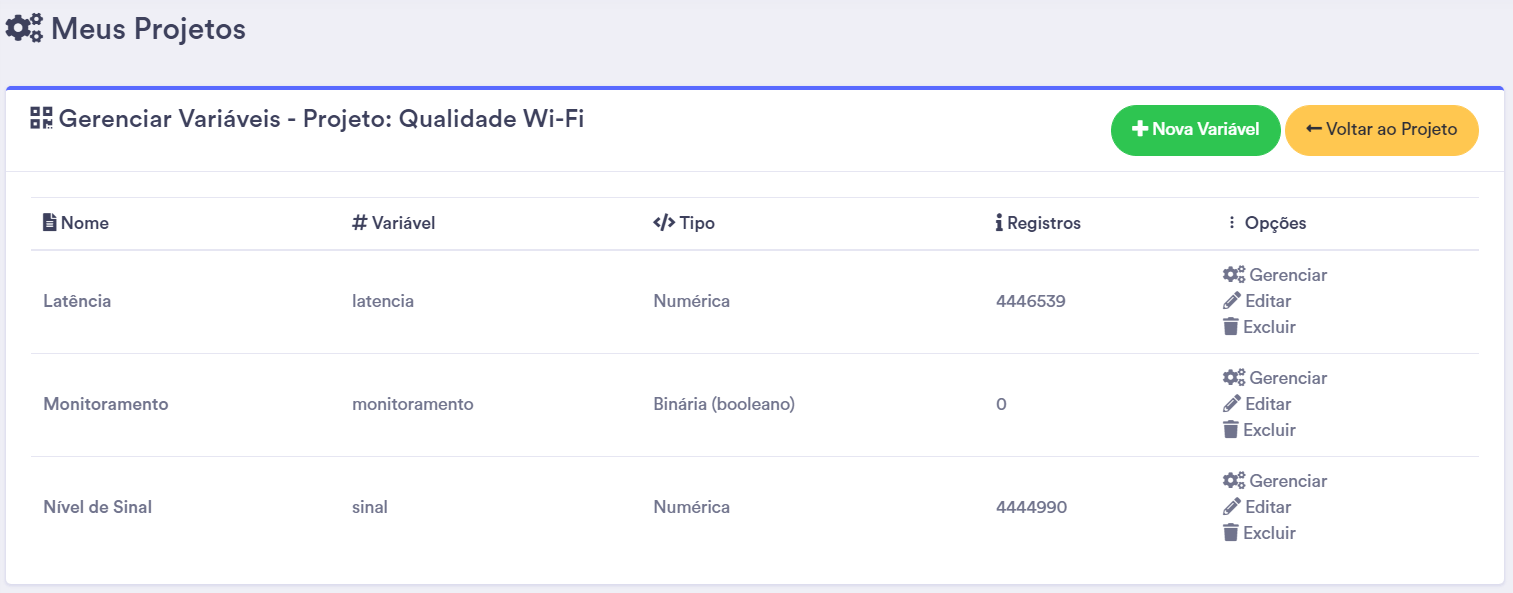
\includegraphics[width=15cm]{figuras/wifi-variaveis.png}}
		}{
			\Fonte{O autor}
		}	
    	\end{figure}


Foram utilizados um total de 5 objetos, sendo o primeiro, uma chave para ligar ou desligar o monitoramento do exemplo, duas do tipo Último Valor para demonstrar os valores instantâneos recebidos pelo microcontrolador e suas variações, representados na Figura \ref{fig:figura-wifi-instataneos} e outros 2 do tipo gráfico, para acompanhar a variação das informações através do tempo em uma janela de tempo configurada com 10 minutos de período. 

        \begin{figure}[!h]
		\Caption{\label{fig:figura-wifi-instataneos} Botão para ação no processo além de últimas informações enviadas.}
		%\centering
		\UFCfig{}{
			\fbox{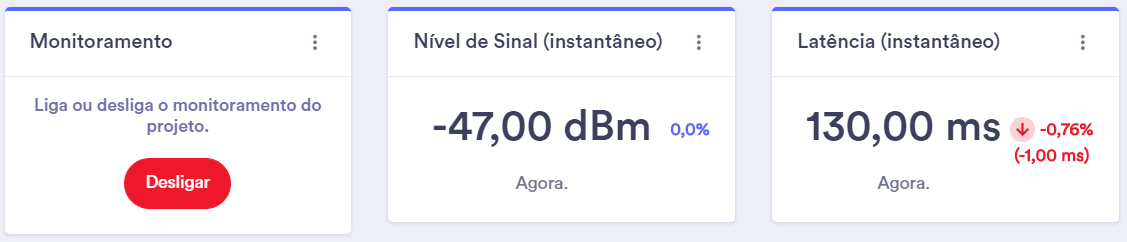
\includegraphics[width=15cm]{figuras/wifi-instataneos.png}}
		}{
			\Fonte{O autor}
		}	
    	\end{figure}
    	
Para o período de captura utilizado neste exemplo, na Figura \ref{fig:figura-wifi-sinal}, houve uma variação na potência do sinal recebido pelo microcontrolador com um intervalo entre -55 dBm e -38 dBm. O Gráfico da latência da conexão, representado na Figura \ref{fig:figura-wifi-latencia}, assim como no exemplo da seção \ref{sec:temperatura-umidade}, houve um aumento na latência entre 19h52 e 19h54 do dia em que a captura foi feita, provavelmente devido ao pico de demanda do provedor neste horário já que imediatamente na figura anterior podemos constatar que não houveram variações bruscas no sinal da rede interna.
    	
        \begin{figure}[!h]
		\Caption{\label{fig:figura-wifi-sinal} Gráfico de linhas com os últimos 30 minutos de qualidade de sinal registrada.}
		%\centering
		\UFCfig{}{
			\fbox{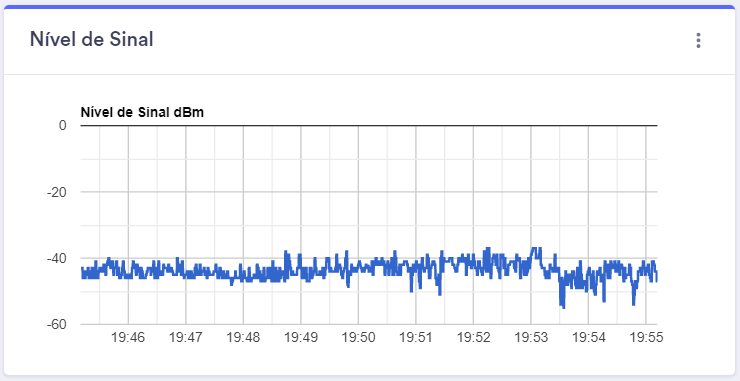
\includegraphics[width=10cm]{figuras/wifi-sinal.png}}
		}{
			\Fonte{O autor}
		}	
    	\end{figure}
    	
        \begin{figure}[!h]
		\Caption{\label{fig:figura-wifi-latencia} Gráfico de linhas com os últimos 10 minutos de latência registrada.}
		%\centering
		\UFCfig{}{
			\fbox{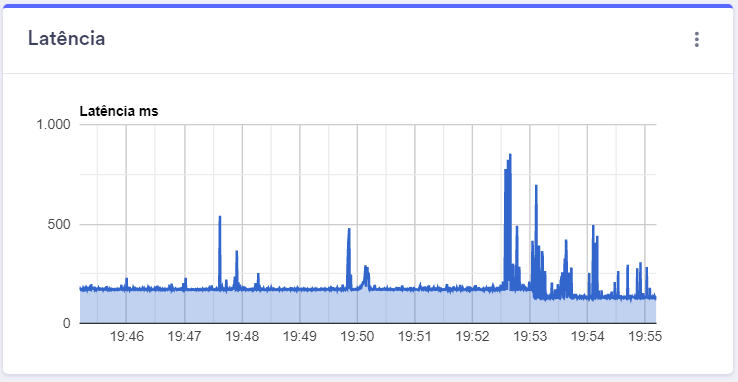
\includegraphics[width=10cm]{figuras/wifi-latencia.png}}
		}{
			\Fonte{O autor}
		}	
    	\end{figure}
    	


\section{Incubadora Neonatal}
\label{sec:incubadora-neonatal}
Com o objetivo de exemplificar uma possível integração entre o sistema \gls{SCADA} proposto e outros sistemas já existentes no local em que seja utilizado, foi desenvolvido um código utilizando o \textit{software} MATLAB, da empresa MathWorks, disponível no anexo \ref{an:anexo-incubadora-neonatal}, para servir como intermediário entre sensores disponibilizados dentro de uma incubadora neonatal e a interface de gerenciamento, similarmente ao que aconteceria caso o cliente optasse pelo uso de um servidor \gls{OPC} local. Utilizou-se a incubadora neonatal presente no Laboratório de Controle, Automação e Telecomunicações da Universidade Federal do Piauí, representada na Figura \ref{fig:figura-incubadora-ela}.

        \begin{figure}[!h]
		\Caption{\label{fig:figura-incubadora-ela} Incubadora utilizada no exemplo.}
		%\centering
		\UFCfig{}{
			\fbox{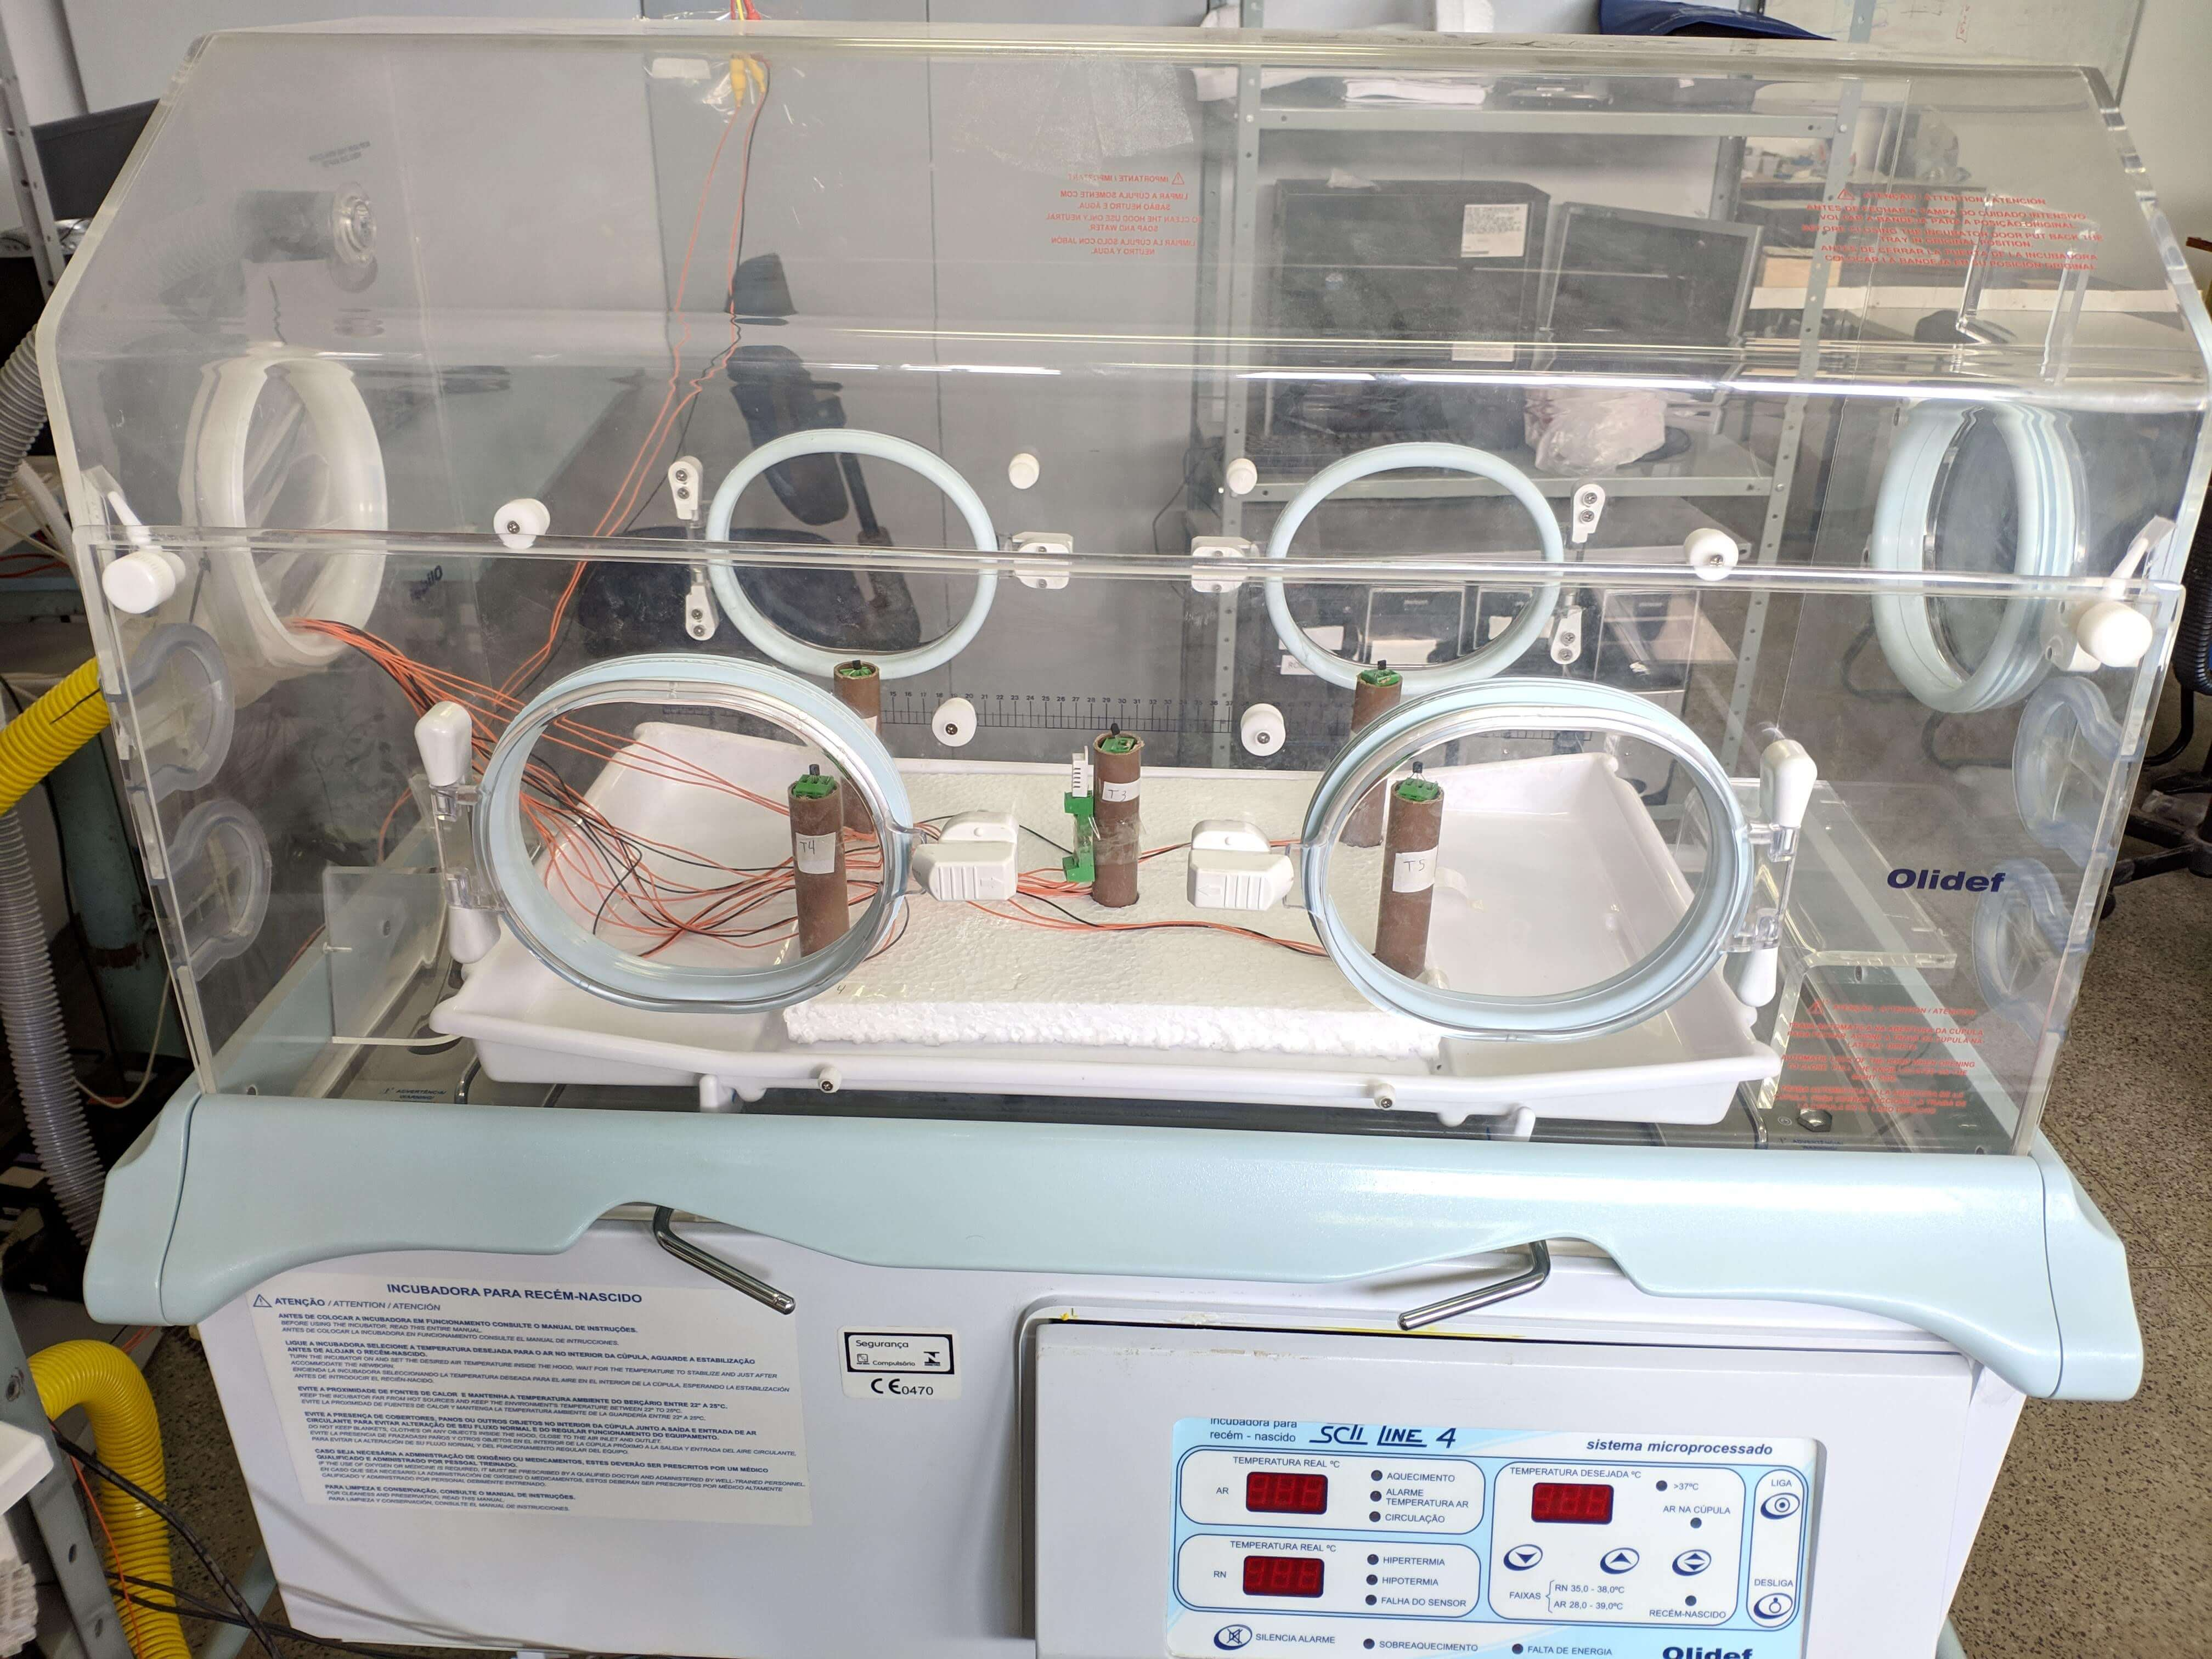
\includegraphics[width=10cm]{figuras/incubadora-ela.jpg}}
		}{
			\Fonte{O autor}
		}	
    	\end{figure}
    	
Os sensores são dispostos dentro da cúpula, conforme a Figura \ref{fig:figura-incubadora-pontos} seguindo a norma NBR IEC 60601-2-19/2014. Neste exemplo, foram capturadas informações de temperatura através de sensores localizados: (i) no ponto M, que representam a média da temperatura interna na cúpula, (ii) próximo a resistência interna, responsável pelo aquecimento da incubadora através da passagem de corrente elétrica  e, (iii) posicionado para medição da temperatura externa.
    	
        \begin{figure}[!h]
		\Caption{\label{fig:figura-incubadora-pontos} Pontos em que os sensores são posicionados.}
		%\centering
		\UFCfig{}{
			\fbox{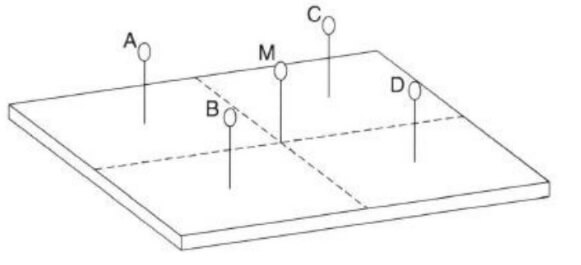
\includegraphics[width=10cm]{figuras/incubadora-pontos.jpg}}
		}{
			\Fonte{(NBR IEC 60601-2-19, 2014)}
		}	
    	\end{figure}
    	
Inicialmente foram configuradas as variáveis à serem utilizadas pelo exemplo, sendo elas:
\begin{alineascomponto}
    \item Referência Temperatura: tipo numérica que representa o sinal base de entrada para a resistência;
    \item Temperatura: tipo numérica representando a temperatura na resistência interna da incubadora;
    \item Temperatura Cúpula: tipo numérica para a temperatura interna da cúpula, representada na Figura \ref{fig:figura-incubadora-pontos} pelo ponto M;
    \item Temperatura Externa: tipo numérica para captura da temperatura ambiente;
    \item Umidade: tipo numérica para captura da umidade dentro da incubadora;
    \item PWM: tipo numérica que representa o sinal de entrada para a resistência no momento da captura de umidade.
\end{alineascomponto}

A Figura \ref{fig:figura-incubadora-variaveis} traz uma captura da tela de gerenciamento de variáveis, com o exemplo já em funcionamento em duas etapas distintas: (i) Captura de Temperatura, com 80 pontos em suas respectivas variáveis e (ii) Captura de Umidade, com 524 pontos, coletadas a cada 220 segundos.
    	
        \begin{figure}[!h]
		\Caption{\label{fig:figura-incubadora-variaveis} Variáveis utilizadas no projeto.}
		%\centering
		\UFCfig{}{
			\fbox{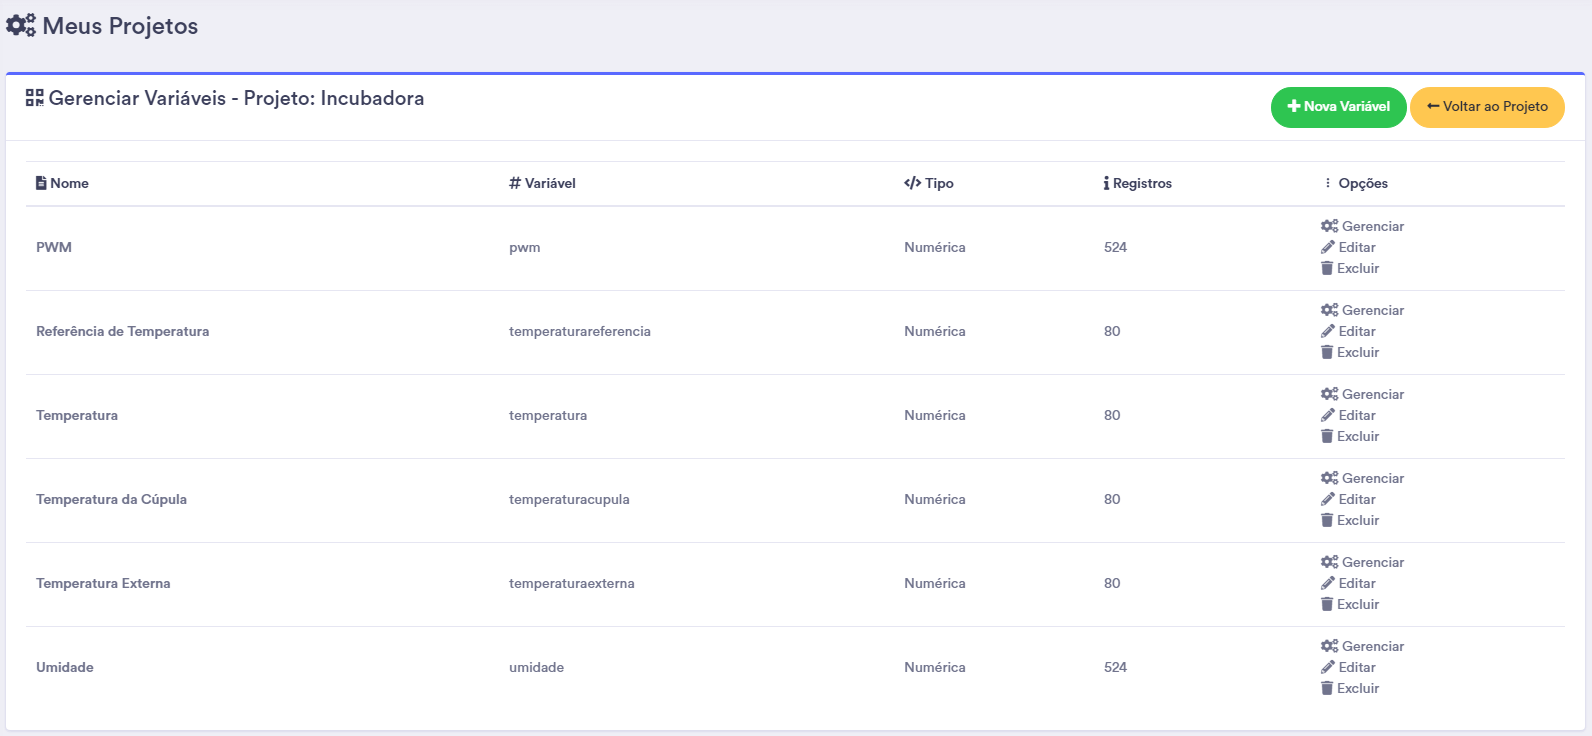
\includegraphics[width=15cm]{figuras/incubadora-variaveis.png}}
		}{
			\Fonte{O autor}
		}	
    	\end{figure}
    	
As Figuras \ref{fig:figura-incubadora-temperatura-referencia} e \ref{fig:figura-incubadora-temperatura} são respectivamente a referência de entrada e a temperatura real obtida. Como o objetivo deste exemplo era apenas a aquisição das informações provenientes do processo, não foram aplicadas quaisquer malhas de controle. Na resistência de aquecimento, a temperatura adquirida em regime permanente foi por volta de 55,4 ºC, conforme Figura \ref{fig:figura-incubadora-temperatura}.

        \begin{figure}[!h]
		\Caption{\label{fig:figura-incubadora-temperatura-referencia} Temperatura de referência para a resistência.}
		%\centering
		\UFCfig{}{
			\fbox{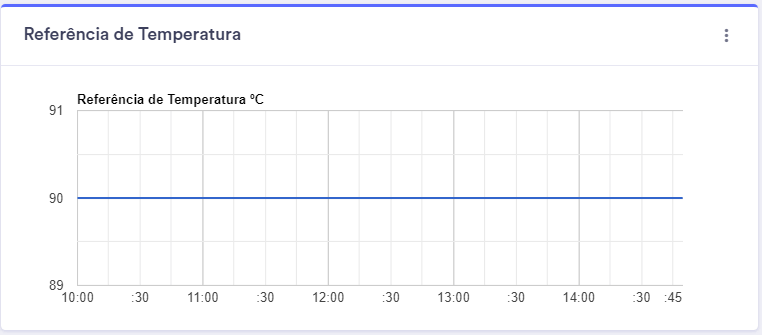
\includegraphics[width=10cm]{figuras/incubadora-temperatura-referencia.png}}
		}{
			\Fonte{O autor}
		}	
    	\end{figure}

Internamente, na cúpula, nos dados obtidos representados pela Figura \ref{fig:figura-incubadora-temperatura-cupula}, a temperatura da resistência se mantém por volta de 42,8 ºC em regime permanente.

        \begin{figure}[!h]
		\Caption{\label{fig:figura-incubadora-temperatura} Curva da temperatura adquirida na resistência.}
		%\centering
		\UFCfig{}{
			\fbox{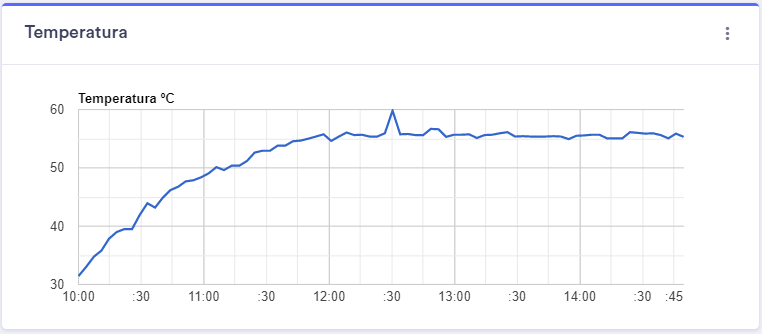
\includegraphics[width=10cm]{figuras/incubadora-temperatura.png}}
		}{
			\Fonte{O autor}
		}	
    	\end{figure}
    	
        \begin{figure}[!h]
		\Caption{\label{fig:figura-incubadora-temperatura-cupula} Curva da temperatura internamente na cúpula.}
		%\centering
		\UFCfig{}{
			\fbox{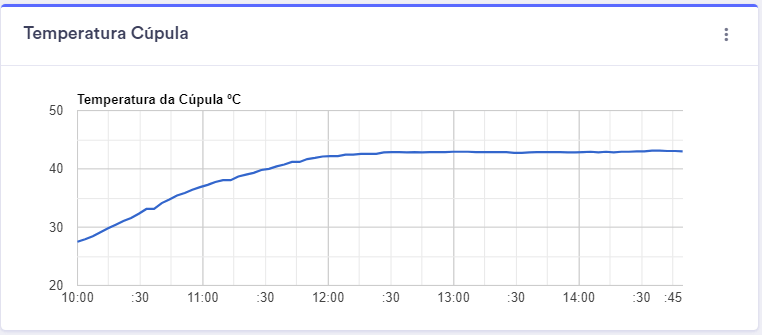
\includegraphics[width=10cm]{figuras/incubadora-temperatura-cupula.png}}
		}{
			\Fonte{O autor}
		}	
    	\end{figure}
    	
A temperatura externa à incubadora (ambiente) no momento da aquisição se mantém oscilando por volta de 30º C, conforme Figura \ref{fig:figura-incubadora-temperatura-externa}. A Figura \ref{fig:figura-incubadora-umidade} representa a curva de umidade para a segunda etapa de captura da incubadora.

    	\begin{figure}[!h]
		\Caption{\label{fig:figura-incubadora-temperatura-externa} Curva da temperatura externa no momento da aquisição.}
		%\centering
		\UFCfig{}{
			\fbox{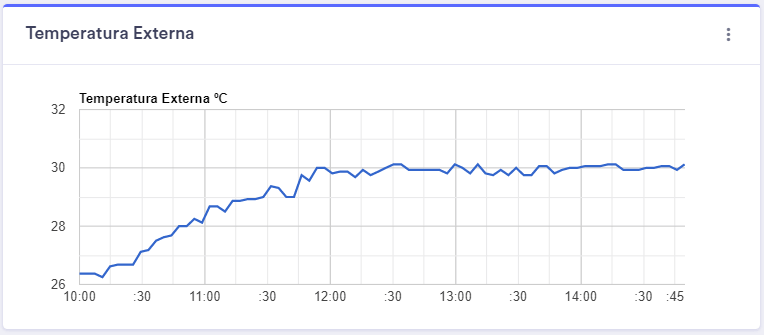
\includegraphics[width=10cm]{figuras/incubadora-temperatura-externa.png}}
		}{
			\Fonte{O autor}
		}	
    	\end{figure}
    	
    	\begin{figure}[!h]
		\Caption{\label{fig:figura-incubadora-umidade} Curva de umidade adquirida.}
		%\centering
		\UFCfig{}{
			\fbox{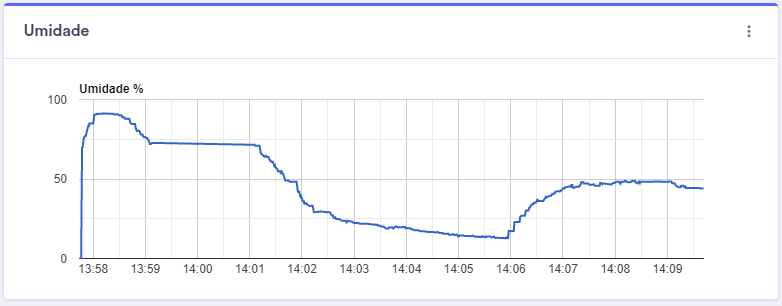
\includegraphics[width=10cm]{figuras/incubadora-umidade.png}}
		}{
			\Fonte{O autor}
		}	
    	\end{figure}
    	

\section{Demanda de Roteadores}
\label{sec:demanda-roteadores}
Para exemplificar a aquisição de dados através do protocolo \gls{HTTP} e uma possível integração entre o sistema \gls{SCADA} proposto e outros sistemas já existentes no local em que seja utilizado, assim como o exemplo anterior, foi desenvolvido um código utilizando a linguagem de programação PHP, disponível no anexo \ref{an:anexo-roteadores}, para o monitoramento de 11 roteadores dispostos no Entre Rios Hotel na cidade de Picos - Piauí. A ideia deste exemplo é ter um histórico de demanda de hóspedes conectados e a máxima largura de banda utilizada em cada um dos roteadores num período de 24 horas, que se situam em locais distintos. Com isso, é possível a reorganização destes aparelhos para um melhor atendimento dos clientes, considerando que haja uma maior demanda na maior parte do tempo em um zona específica do hotel.

Inicialmente foram configuradas as variáveis à serem utilizadas pelo programa, sendo elas:

\begin{alineascomponto}
    \item Apartamento X - \textit{Downlink}, para a aquisição da máxima largura de banda de \textit{download} demandada no período;
    \item Apartamento X - \textit{Download}, para a aquisição da quantidade de dados trafegados em \textit{download} no período;
    \item Apartamento X - \textit{Uplink}, para a aquisição da máxima largura de banda de \textit{uplink} demandada no período;
    \item Apartamento X - Upload, para a aquisição da quantidade de dados trafegados em \textit{upload} no período e, por fim,
    \item Apartamento X - Usuários Ativos para a aquisição da quantidade de hóspedes conectados em dado roteador.
\end{alineascomponto}

Todas variáveis do tipo numérica, em que X nestas variáveis representam o código do roteador à ser monitorado. A Figura \ref{fig:figura-roteadores-variaveis} traz uma captura da tela de gerenciamento de variáveis, com o exemplo do primeiro roteador, localizado próximo ao apartamento 103, contando com algo em torno de 15 mil registros por variável no momento da captura.

        \begin{figure}[!h]
		\Caption{\label{fig:figura-roteadores-variaveis} Variáveis utilizadas no projeto.}
		%\centering
		\UFCfig{}{
			\fbox{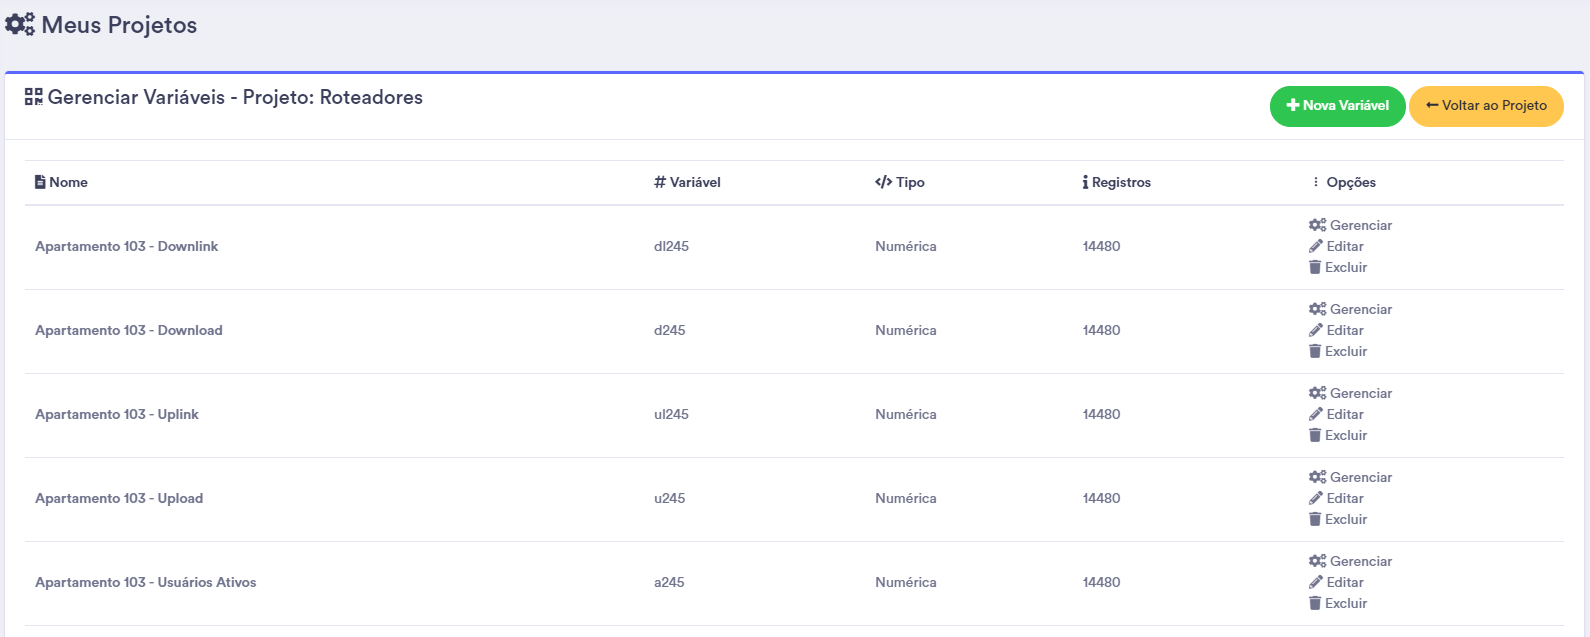
\includegraphics[width=15cm]{figuras/roteadores-variaveis.png}}
		}{
			\Fonte{O autor}
		}	
    	\end{figure}
    	
        \begin{figure}[!h]
		\Caption{\label{fig:figura-roteadores-recepcao} Quantidade de hóspedes conectados no roteador da recepção durante 24 horas.}
		%\centering
		\UFCfig{}{
			\fbox{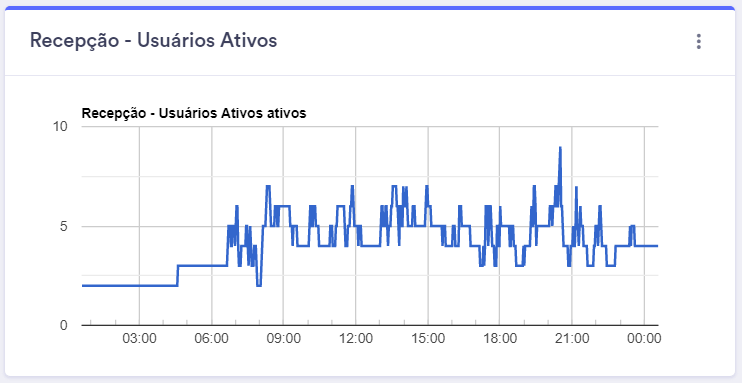
\includegraphics[width=10cm]{figuras/roteadores-recepcao.png}}
		}{
			\Fonte{O autor}
		}	
    	\end{figure}
    	
Foram utilizados um total de 22 objetos para este exemplo, todos do tipo Gráfico de Linha, para a plotagem da quantidade de hóspedes conectados por roteador, representados pelas Figuras \ref{fig:figura-roteadores-recepcao} e \ref{fig:figura-roteadores-107} e, a máxima largura de banda de \textit{download} em cada um deles, Figuras \ref{fig:figura-roteadores-recepcao-downlink} e \ref{fig:figura-roteadores-107-downlink}, roteadores da Recepção e próximo ao apartamento 107 respectivamente.

        \begin{figure}[!h]
		\Caption{\label{fig:figura-roteadores-recepcao-downlink} Uso máximo de downlink pelo roteador da recepção durante 24 horas.}
		%\centering
		\UFCfig{}{
			\fbox{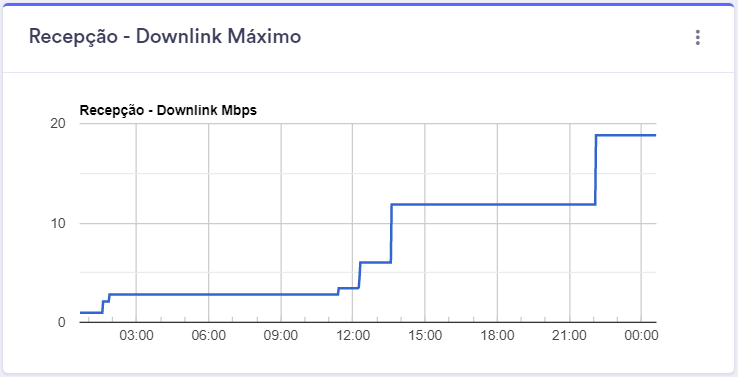
\includegraphics[width=10cm]{figuras/roteadores-recepcao-downlink.png}}
		}{
			\Fonte{O autor}
		}	
    	\end{figure}
    	
A Figura \ref{fig:figura-roteadores-recepcao} traz o pico máximo de 9 hóspedes conectados no roteador da Recepção neste dia, enquanto que na Figura \ref{fig:figura-roteadores-recepcao-downlink}, é possível ver um aumento gradativo da máxima largura de banda de \textit{download} diária, onde o máximo para o período de 24 horas foi de aproximadamente 18 Mbps.

        \begin{figure}[!h]
		\Caption{\label{fig:figura-roteadores-107} Quantidade de hóspedes conectados no roteador "107" durante 24 horas.}
		%\centering
		\UFCfig{}{
			\fbox{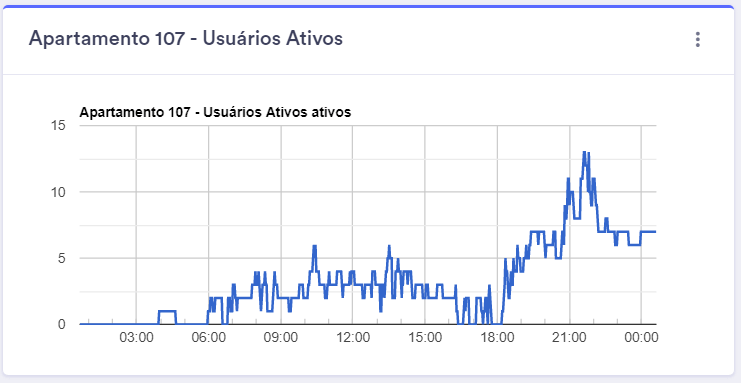
\includegraphics[width=10cm]{figuras/roteadores-107.png}}
		}{
			\Fonte{O autor}
		}	
    	\end{figure}
    	
A mesma análise pode ser realizada para os arredores do apartamento 107, a Figura \ref{fig:figura-roteadores-107}, mostra um pico de 13 hóspedes conectados neste dia, enquanto que na Figura \ref{fig:figura-roteadores-107-downlink}, é possível perceber uma máxima largura de banda de \textit{download} diária em torno de 30 Mbps.

        \begin{figure}[!h]
		\Caption{\label{fig:figura-roteadores-107-downlink} Uso máximo de downlink pelo roteador "107" durante 24 horas.}
		%\centering
		\UFCfig{}{
			\fbox{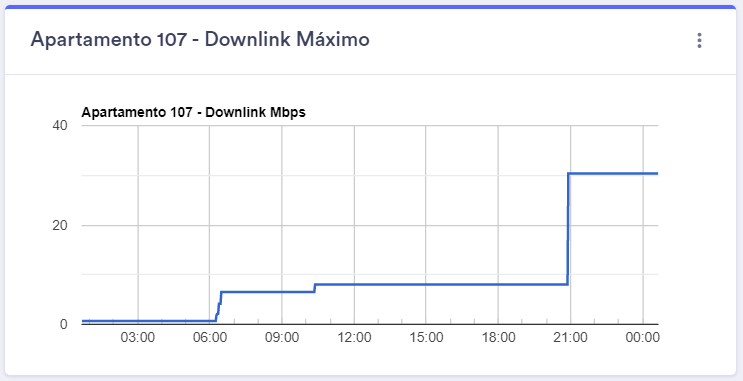
\includegraphics[width=10cm]{figuras/roteadores-107-downlink.png}}
		}{
			\Fonte{O autor}
		}	
    	\end{figure}